\documentclass[tikz,border=8pt]{standalone}
\usetikzlibrary{shapes.geometric, arrows.meta, positioning, fit
, calc}

\usepackage{tikz}
\usetikzlibrary{arrows.meta, positioning}



\tikzset{
  process/.style = {rectangle, rounded corners=3pt,
                    draw=black, very thick,
                    minimum width=3.5cm, minimum height=1.1cm,
                    align=center, font=\small, fill=gray!10},
  group/.style   = {draw, dashed, inner sep=4pt, rounded corners=3pt},
  ->/.style      = {thick, -{Stealth[length=6pt,width=7pt]}}
}

\begin{document}

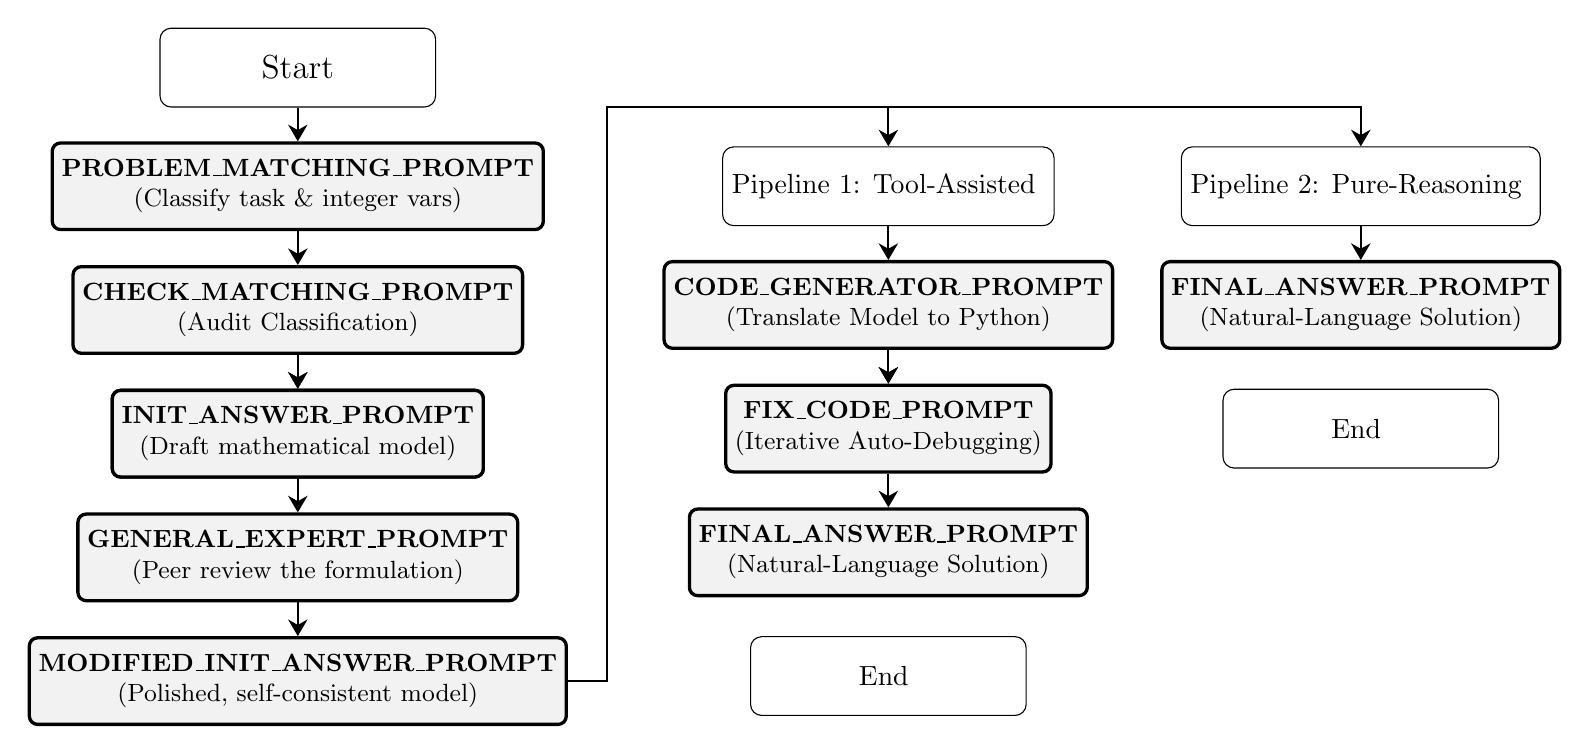
\begin{tikzpicture}[
    node distance=1.5cm and 2.5cm,
    box/.style={draw, rounded corners, minimum width=3.5cm, minimum height=1cm, align=center},
    every edge/.style={draw, -{Latex[length=2mm]}},
    process/.style = {rectangle, rounded corners=3pt,
                    draw=black, very thick,
                    minimum width=3.5cm, minimum height=1.1cm,
                    align=center, font=\small, fill=gray!10},
    group/.style   = {draw, dashed, inner sep=4pt, rounded corners=3pt},
    ->/.style      = {thick, -{Stealth[length=6pt,width=7pt]}}
]

% Shared front-end
% \node[box] (start) {Start};
\node[draw, box] at (0, 0) (start) {\large Start};

\node[ draw, box, align=center, process
] at ($(start.south) + (0cm, -1cm)$) (step1) {
    \textbf{PROBLEM\_MATCHING\_PROMPT}\\(Classify task \& integer vars)
};

\draw[->] (start) -> (step1);

\node[ draw, box, align=center, process
] at ($(step1.south) + (0cm, -1cm)$) (step2) {
    \textbf{CHECK\_MATCHING\_PROMPT}\\(Audit Classification)
};

\draw[->] (step1) -> (step2);

\node[ draw, box, align=center, process
] at ($(step2.south) + (0cm, -1cm)$) (step3) {
    \textbf{INIT\_ANSWER\_PROMPT}\\(Draft Model)
};

\draw[->] (step2) -> (step3);
\node[ draw, box, align=center, process
] at ($(step2.south) + (0cm, -1cm)$) (step3) {
    \textbf{INIT\_ANSWER\_PROMPT}\\(Draft mathematical model)
};

\draw[->] (step2) -> (step3);

\node[ draw, box, align=center, process
] at ($(step3.south) + (0cm, -1cm)$) (step4) {
    \textbf{GENERAL\_EXPERT\_PROMPT}\\(Peer review the formulation)
};

\draw[->] (step3) -> (step4);

\node[ draw, box, align=center, process
] at ($(step4.south) + (0cm, -1cm)$) (step5) {
    \textbf{MODIFIED\_INIT\_ANSWER\_PROMPT}\\(Polished, self-consistent model)
};

\draw[->] (step4) -> (step5);

\node[ draw, box, align=center
] at ($(start.south) + (7.5cm, -1cm)$) (step6) {
    Pipeline 1: Tool-Assisted
};

\draw[->] (step5.east) -- ++(0.5, 0) |- ($(step6.north) + (0cm, 0.5cm)$) -| (step6.north);

\node[ draw, box, align=center, process
] at ($(step6.south) + (0cm, -1cm)$) (step7) {
    \textbf{CODE\_GENERATOR\_PROMPT}\\(Translate Model to Python)
};

\draw[->] (step6) -> (step7);

\node[ draw, box, align=center, process
] at ($(step7.south) + (0cm, -1cm)$) (step8) {
    \textbf{FIX\_CODE\_PROMPT}\\(Iterative Auto-Debugging)
};

\draw[->] (step7) -> (step8);

\node[ draw, box, align=center, process
] at ($(step8.south) + (0cm, -1cm)$) (step9) {
    \textbf{FINAL\_ANSWER\_PROMPT}\\(Natural-Language Solution)
};

\draw[->] (step7) -> (step8);

\draw[->] (step8) -> (step9);

\node[ draw, box, align=center
] at ($(start.south) + (13.5cm, -1cm)$) (step10) {
    Pipeline 2: Pure-Reasoning
};

\draw[->] ($(step5.east) + (0cm, 0cm)$) 
    -| ($(step5.east) + (0.5cm, 0cm)$) 
    |- ($(step10.north) + (0cm, 0.5cm)$) 
    -| (step10.north)
;

\node[ draw, box, align=center, process
] at ($(step10.south) + (0cm, -1cm)$) (step11) {
    \textbf{FINAL\_ANSWER\_PROMPT}\\(Natural-Language Solution)
}; 

\draw[->] (step10) -> (step11);

\node[draw, box, align=center
] at ($(step11.south) + (0cm, -1cm)$) (end) {
    End
};

\node[draw, box, align=center
] at ($(step9.south) + (0cm, -1cm)$) (end2) {
    End
};




\end{tikzpicture}
\end{document}
